\chapter{Experiments}
%Basic Environments, PickPlace is harder than reach etc., Plappert et. al., HER paper..

This chapter describes the experiments that were carried out and their results. This chapter is divided into 3 subchapters.
%change number of chapters if it changes
\newline
First the four robotics environments "FetchReach", "FetchPush", "FetchSlide" and "FetchPickAndPlace" that are already integrated in OpenAI Gym, will be compared and used as benchmarks.
%ref Plappert et al.
Then two self created environments, FetchSlideball and FetchToss will be described.
\vspace{0.5cm}

"FetchSlideball" is an extension of FetchSlide. We changed the object from a cylinder to a ball and increased the distance to the goal. This will be compared with the FetchSlide environment of the benchmarks. It is planned to improve this environment to an environment that simulates a golf course in the future.
\vspace{0.5cm}

"FetchToss" requires the agent to toss an object to a goal that is outside of the agents reach. It requires the agent to grab the object and then find the right trajectory to move the object and release it to toss it. The first part of the task is comparable to FetchPickAndPlace that requires the fetch robot to fetch the object. It was planned to improve this environment to make it toss a ball into a basket like in basketball.
\vspace{0.5cm}

In each chapter, the tasks and environment will be described. The action space, observation space and rewards to control the agent are also described. Then the results are discussed and compared to other tasks.   

%We want to have golf/basketball , so we use a ball instead
%We change the distance
%doesnt work because too far, maybe also reasons from HGG
%change friction
%interesting results, cheating v9
%use v9 on v2 is not bad, show v5
%(do v9 with wall)
%basketball
%throwing, doesnt work, too hard
%throwing ball also
%put wall, maybe it throws over goal
%try longer timesteps
%try putting box closer

\section{Fetch environments by OpenAI}

In this section, the four basic robotics environments of OpenAI with the fetch robotic arm are shortly described and compared.

\subsection{FetchReach}

\begin{figure} [h]
	
	\centering
	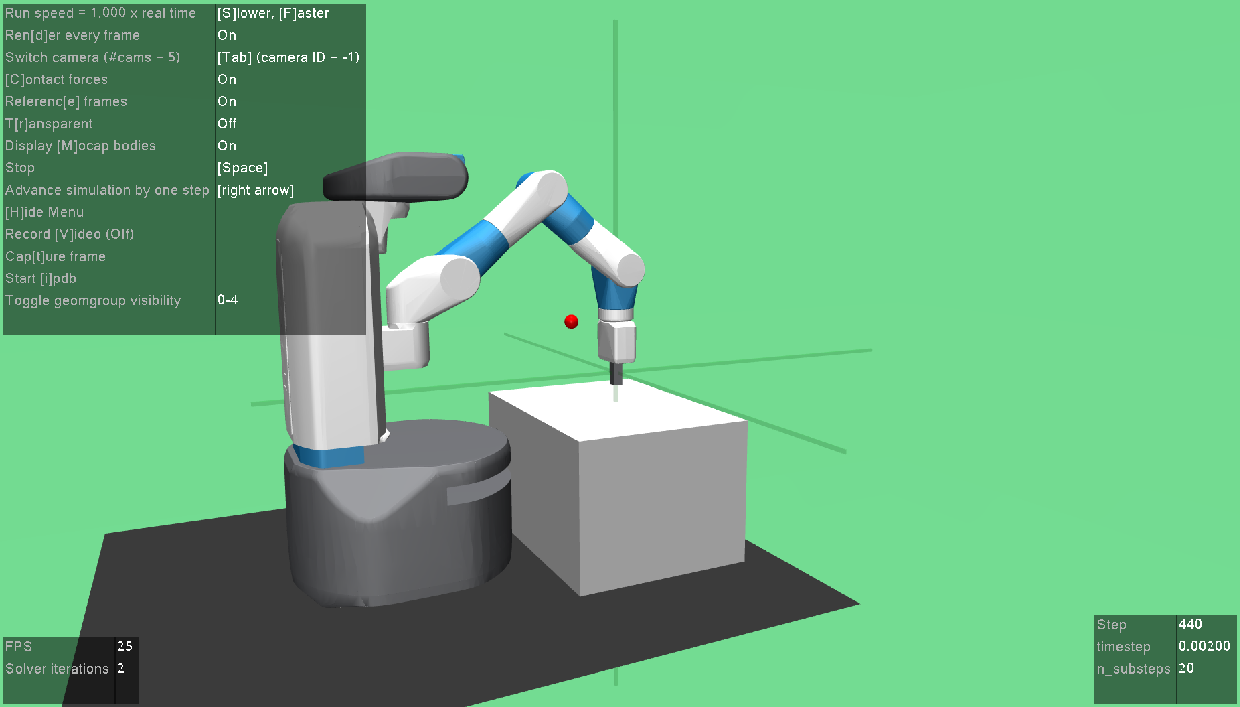
\includegraphics[width=1\textwidth]{figures/FetchReach-v1.pdf}
	\caption{FetchReach-v1}
	\label{reach1}
\end{figure} 

The environment FetchReach is the simplest of the OpenAI robotic environments. As can be seen in figure \ref{reach1}, the environment consists of the fetch robot, a table and a red ball indicating the goal. The task is to make the robot move its gripper to the same position as the goal. The goal can be on the table as well as in the air. Also, the goal is only above the table, so the robot is always able to reach the goal. The only thing the robot has to figure out is a path from one starting point to different points.

\vspace{0.5cm}

Figure \ref{benchm} shows how effective HER is.  After just about 7 epochs, the success rate is already at 100\%.




\subsection{FetchPush}

\begin{figure} [h]
	
	\centering
	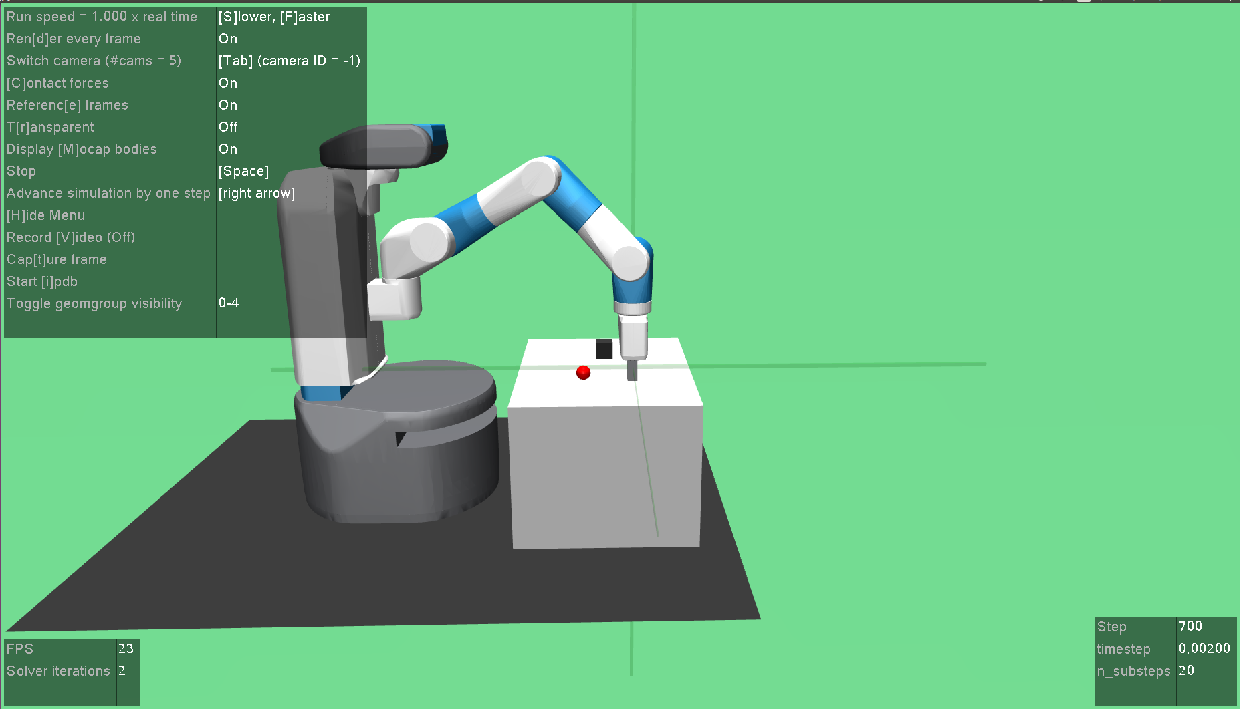
\includegraphics[width=1\textwidth]{figures/FetchPush-v1.pdf}
	\caption{FetchPush-v1}
	\label{push1}
\end{figure}

FetchPush is already much harder than FetchReach. The environment is the same as in FetchReach, but an object in form of a cube was added. This can be seen in figure \ref{push1}. The goal is to move the cube to the goal position. This requires the robot to learn how to move its gripper from the start position to the side of the cube that is away from the goal. Then it needs to move its gripper towards the goal to solve the task. Still, HER proves to be quite powerful. After about 14 epochs, In comparison to FetchReach, it took about twice the time to learn to solve the task.





\subsection{FetchSlide}

\begin{figure} [h]
	
	\centering
	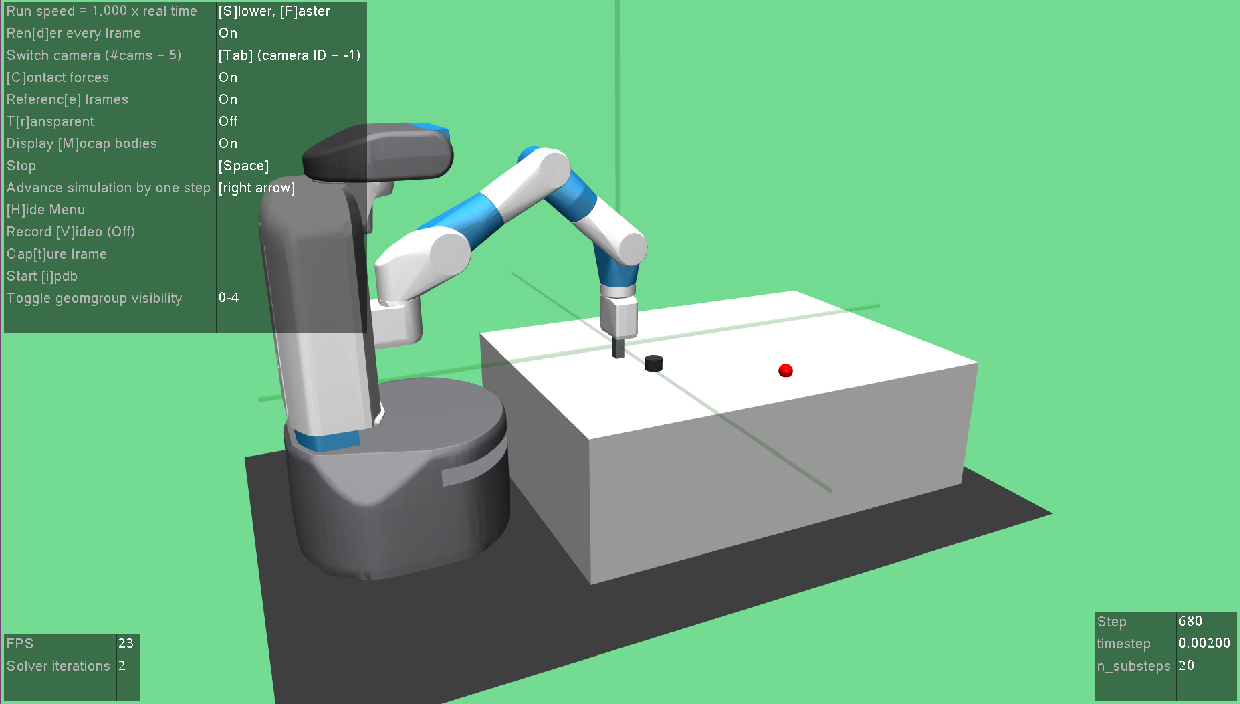
\includegraphics[width=1\textwidth]{figures/FetchSlide-v1.pdf}
	\caption{FetchSlide-v1}
	\label{slide1}
\end{figure}

The FetchSlide environment is quite similar to FetchPush. The task is the same, the robot has to move an object, this time it is a cylinder (similar to a curling stone for curling). There are two main differences to FetchPush which make the task harder. The cylinder has less friction and slides, so the robot needs to carefully move the cylinder to avoid making it slide too far. Also the goal position is further away, partly even outside of the robotic arms' range. So the sliding property of the cylinder has to be used in order to reach those goals. 

\vspace{0.5cm}

Using HER provides worse results than FetchPush. After training, the robot only reaches a success rate of about 60\%. 
In the failed attempts the robot learned to push the cylinder in the right direction, only the distance is not right. The cylinder either slides too far or does not slide far enough. Most of these fails have goal positions that are outside of the robotic arms' range. Interestingly, the robot also struggles with goals that are inside of the robotic arms' range. This is probably due to the sliding property. When touching the cylinder while training, the cylinder will probably slide further away and might often land outside of the robotic arms' reach. With HER, the agent learns to reach the states that it already reached at some point. Because the cylinder has a lot more positions it can be in due to its sliding property, other than in FetchPush, it does not learn to move the cylinder inside its range as well as in FetchPush.    

\subsection{FetchPickAndPlace}

\begin{figure} [h]
	
	\centering
	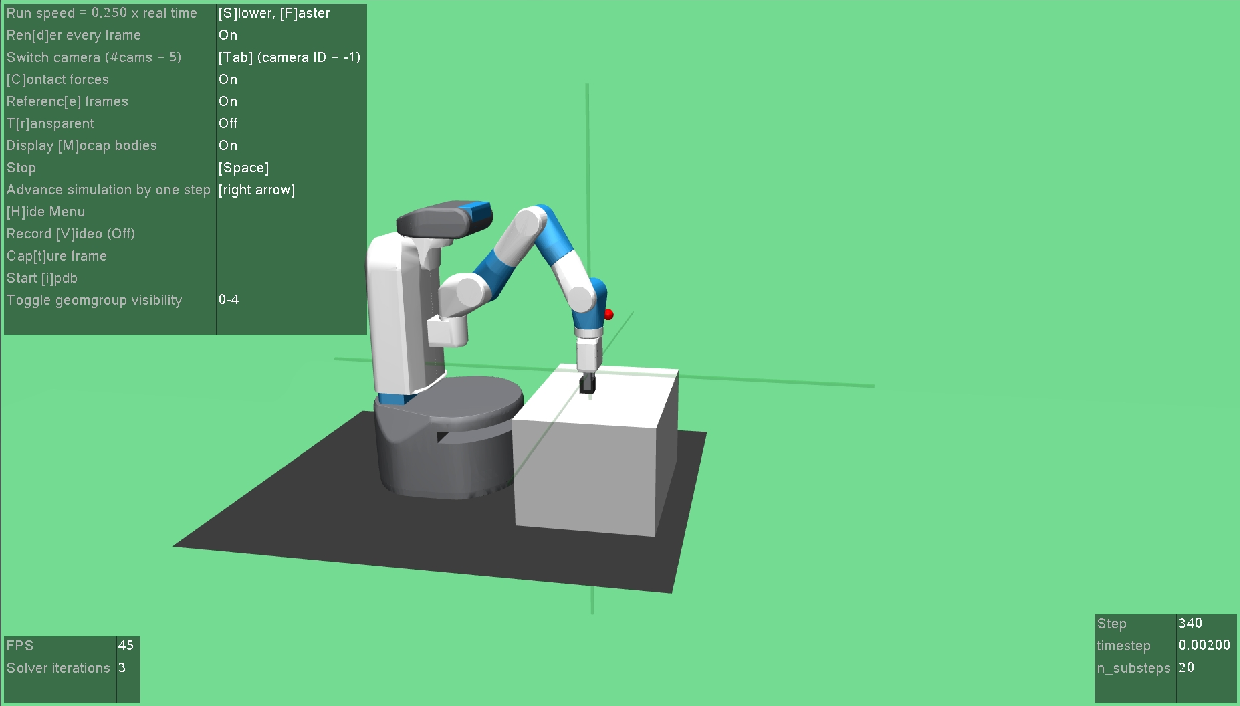
\includegraphics[width=1\textwidth]{figures/FetchPickAndPlace-v1.pdf}
	\caption{FetchPickAndPlace-v1}
	\label{pickplace2}
\end{figure}

The environment for FetchPickAndPlace is exactly the same as in FetchPush except for the goal position. It can also be in the air. This requires the robot to use its gripper to fetch the cube and move it to the goals in the air. So the robot has to learn how to move its gripper towards the cube and open its gripper, then close its gripper to grab the cube. Then it has to move the cube to the goal position without dropping the cube by opening its gripper. 
The training results in figure \ref{benchm} show that learning to solve this task works quite well with HER. After about 30 epochs it almost reaches 100\% success rate. 
%maybe in comparison part
The reason why it takes much more times than the FetchPush task can be explained when comparing both. In the FetchPush task, the agent needs to learn to move its arm to the cube on the side farther away from the goal, then move its arm towards the goal. We have seen in FetchReach that it is quite simple to learn how to move the arm from one position to another. The difficulty in FetchPush comes from figuring out how to move the object. In FetchPickAndPlace this is even harder, because the opening and closing the gripper is also part of the actions it can take. Learning how to grab the cube and keep it grabbed seems to be a the cause to why it takes more time to learn. 


\subsection{Discussion of Results}
%obv. harder tasks take longer and are performing worse
%use Plappert et. al /her paper as reference

\begin{figure} [h]
	
	\centering
	\subfigure[FetchReach-v1] {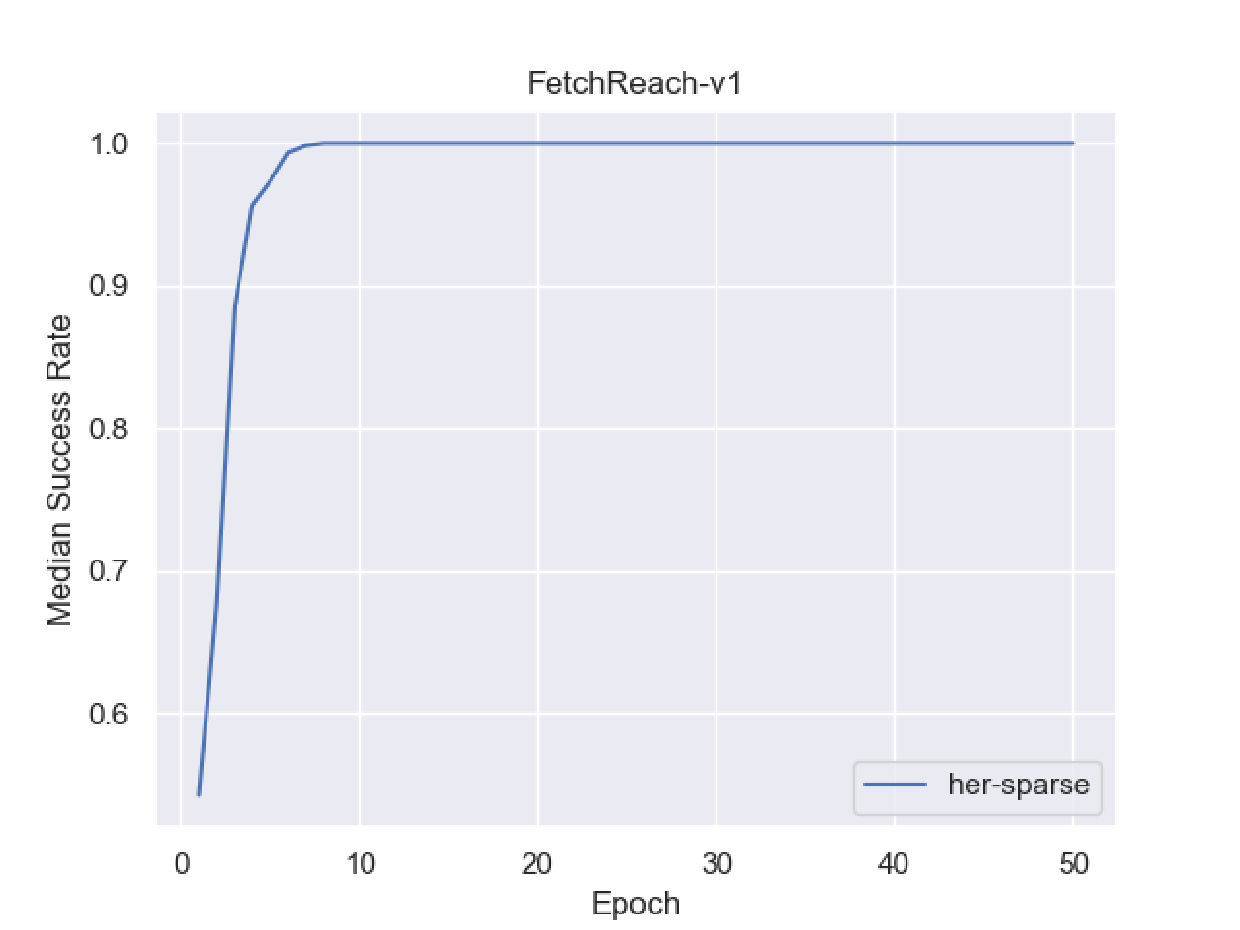
\includegraphics[width=0.49\textwidth]{figures/fig_FetchReach-v1.pdf}\label{fig:fig_fetchreach-v1}}
	\subfigure[FetchPush-v1] {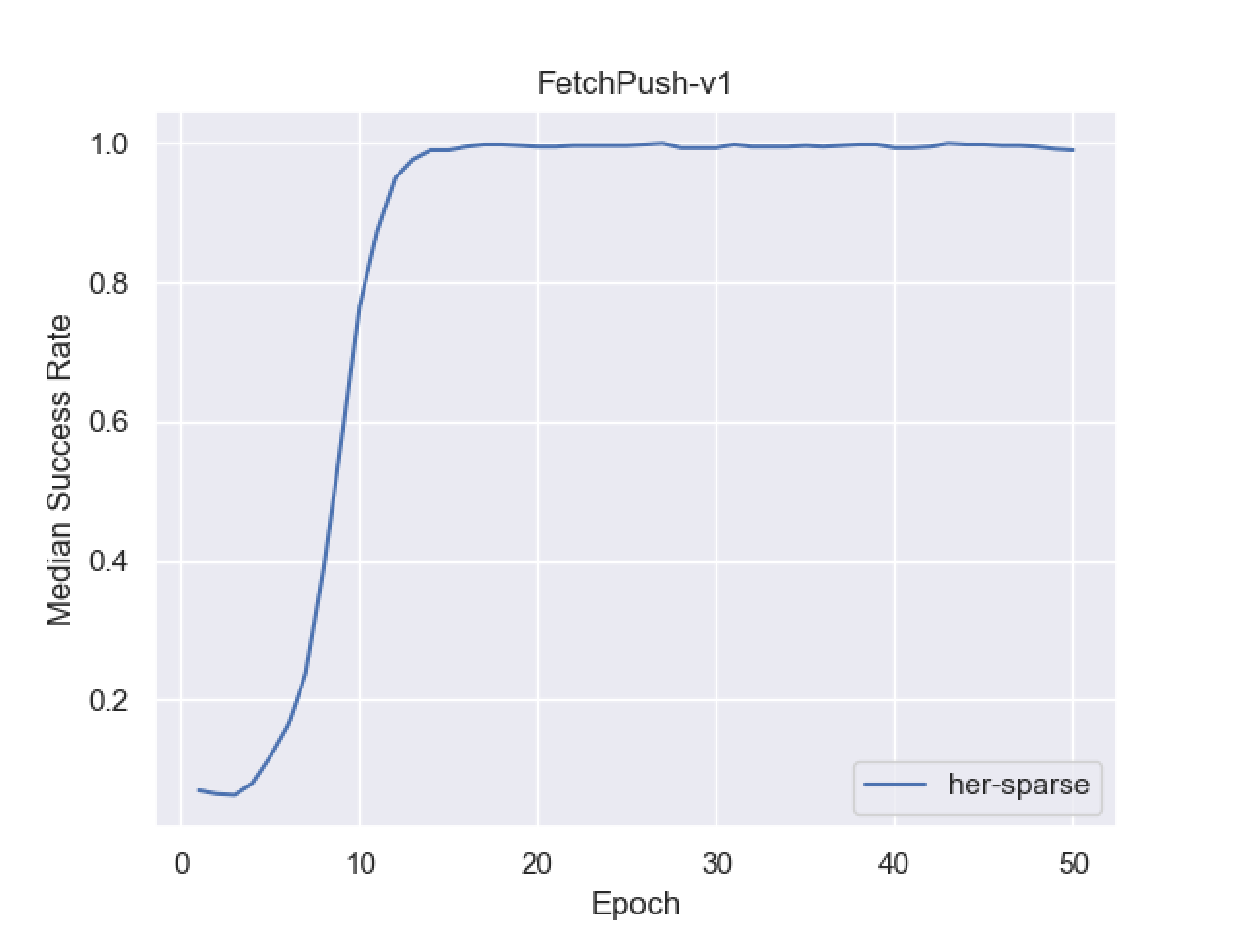
\includegraphics[width=0.49\textwidth]{figures/fig_FetchPush-v1.pdf}\label{fig:fig_fetchpush-v1}}
	\subfigure[FetchSlide-v1] {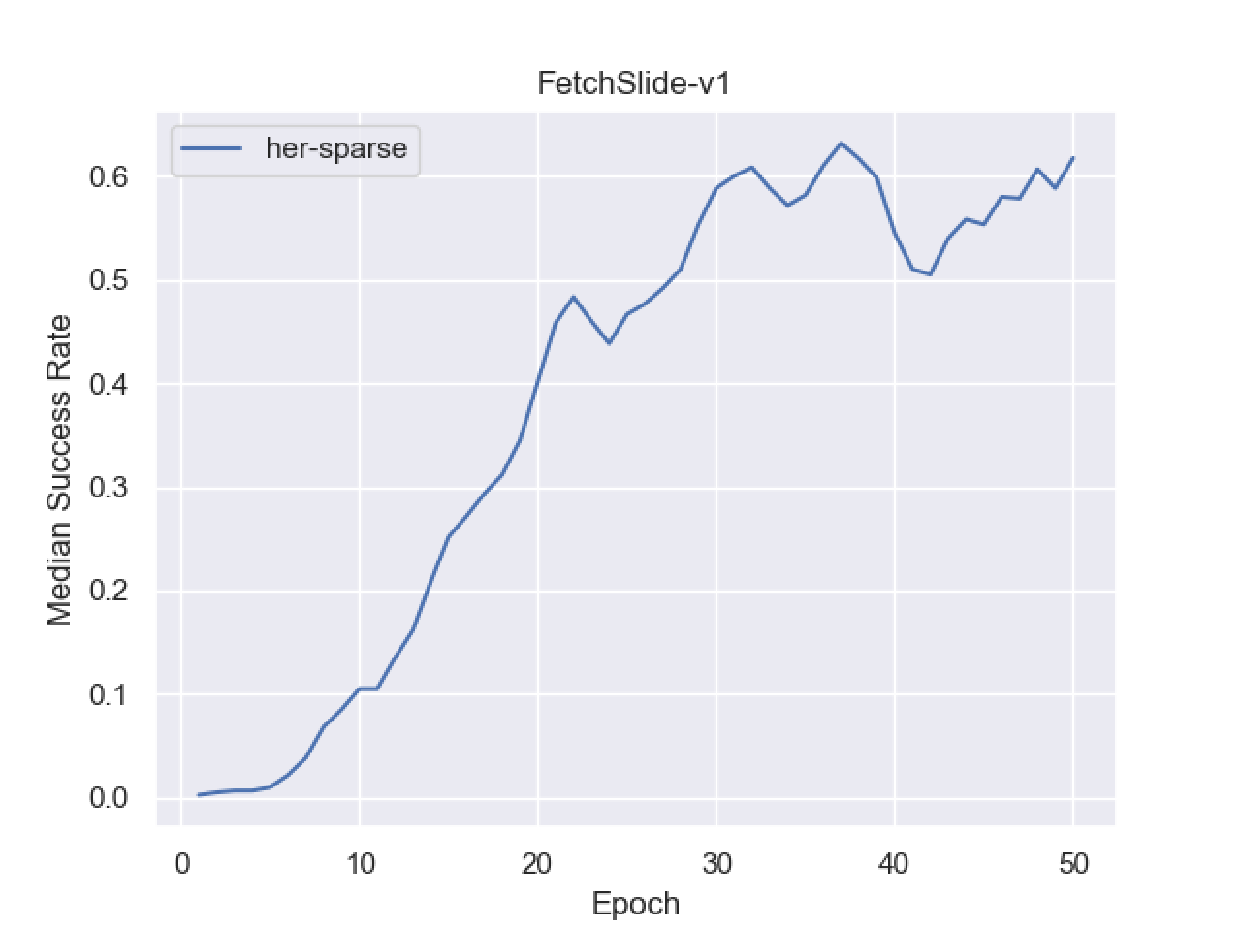
\includegraphics[width=0.49\textwidth]{figures/fig_FetchSlide-v1.pdf}\label{fig:fig_fetchslidea-v1}}
	\subfigure[FetchPickAndPlace-v1] {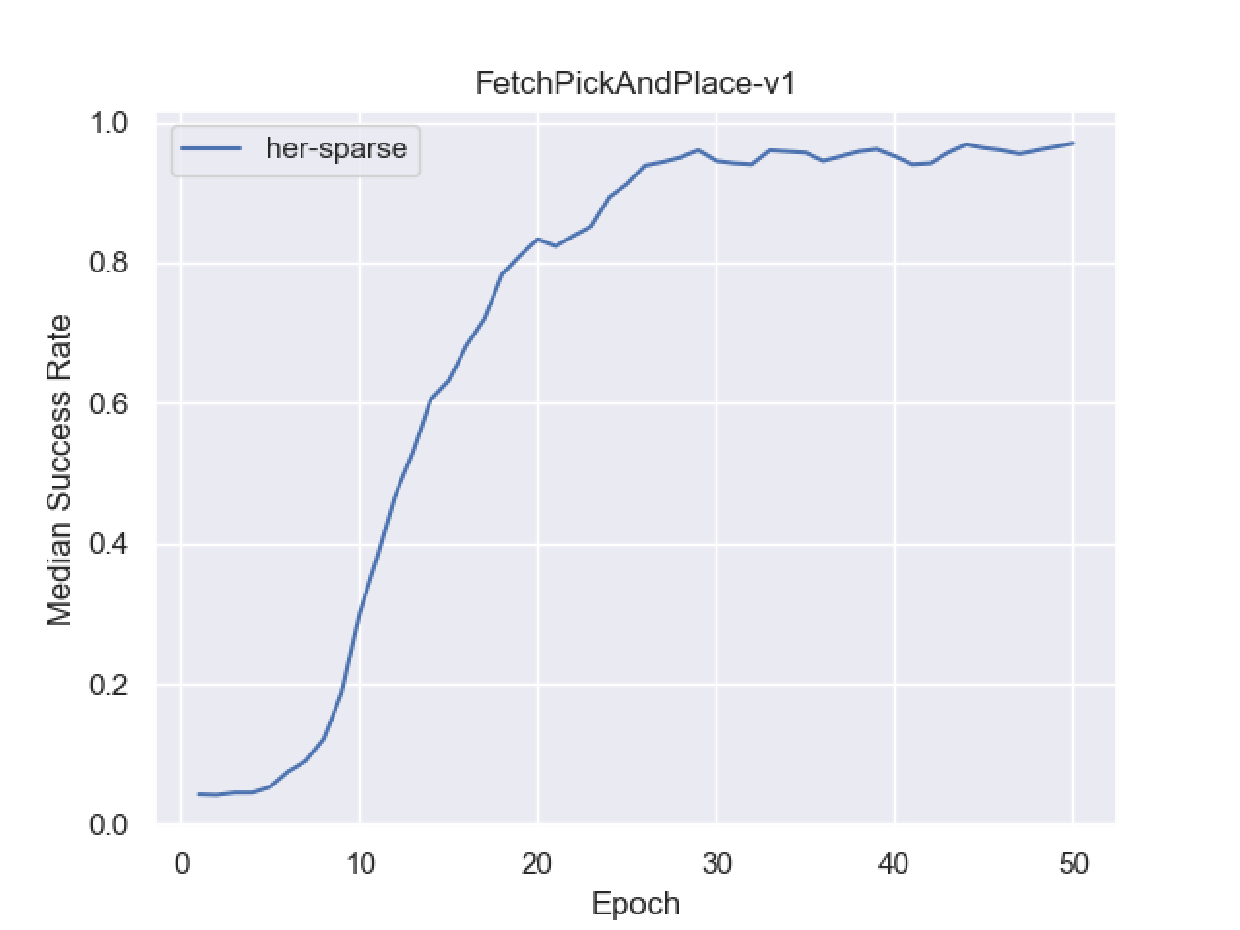
\includegraphics[width=0.49\textwidth]{figures/fig_FetchPickAndPlace-v1.pdf}\label{fig:fig_fetchpickandplace-v1a}}
	\caption{Success Rate of each task after 50 episodes of training}
	\label{benchm}
\end{figure}

Figure \ref{benchm} show the training results for each task.
FetchReach showed that just moving the robotic arm between two points is quite fast and easy to learn.
\newline
Obviously when comparing, the harder tasks FetchSlide and FetchPickAndPlace perform worse than FetchPush and FetchReach. FetchPickAndPlace in comparison to FetchPush introduced the difficulty of having to control opening and closing the gripper. Instead of having an action space with only 3 variables like for the other tasks, this action space is extended to 4 variables, which is an extension of the action space by 33\%. Having to learn how to grab the cube seems to take about 20 episodes longer than not needing to do it. 
%check exact number 
\newline
When comparing FetchSlide to FetchPush, the difference is clear. FetchSlide performs much worse. 
\newline
One difference between both tasks is the control over the object. In FetchSlide it is much harder to control the cylinder while moving it. The robot either has to hit it with very precise force or stop it if the goal position is in the robots' reach. Having big fluctuations between the force used and the distance the cylinder traveled makes it hard to learn how much force exactly is needed. 
\newline
Another difficulty is added by extending the range where the goal can be positioned. These multi-goal environments where the goal and object are in variable positions can be seen as a collection of many simple tasks, where each task is only about moving an object from a fixed position to another. Having a bigger goal space as increases the amount of these simple tasks greatly. As can be seen, these obstacles increase the difficulty drastically. 
%shortly summarize the obstacles ?




\section{FetchSlideball}

FetchSlideball is an extension to the environment FetchSlide. One of the future plans is to have an agent learn how to play golf. FetchSlideball made two differences to FetchSlide: the goal is put even farther in the distance and the cylinder was changed to a ball.
The task will be approached in smaller steps. 
%put this in extra section?
First a simple environment is tested where exactly the same environment as in FetchSlide is used and the only change is for the object to change from a cylinder to a ball. Through this test the difference in difficulty between using a cylinder and a ball is shown. This is needed to make FetchSlideball comparable to FetchSlide. 
Afterwards, for the following experiments, the friction and the steps per episode will be varied. 

\subsection{Task Description}

The task for FetchSlideball is exactly the same as for FetchSlide. The robotic arm has to push a ball from one position to another position, using the balls property to roll farther. Rolling the ball and sliding a cylinder might imply different friction types used, because a ball uses rolling friction instead of sliding friction which is usually much more lower. However, in this environment the same amount of friction is used for both objects. The main difference is the stability of the object. While the cylinder can fall on its side and slide different depending on where it is pushed, the ball stays stable. 
Also, other than in FetchSlide, the goal position is guaranteed to be outside the robots' reach. This should make it much harder for the agent to learn how to solve task.


\subsection{Environment}

\begin{figure} [!h]
	
	\centering
	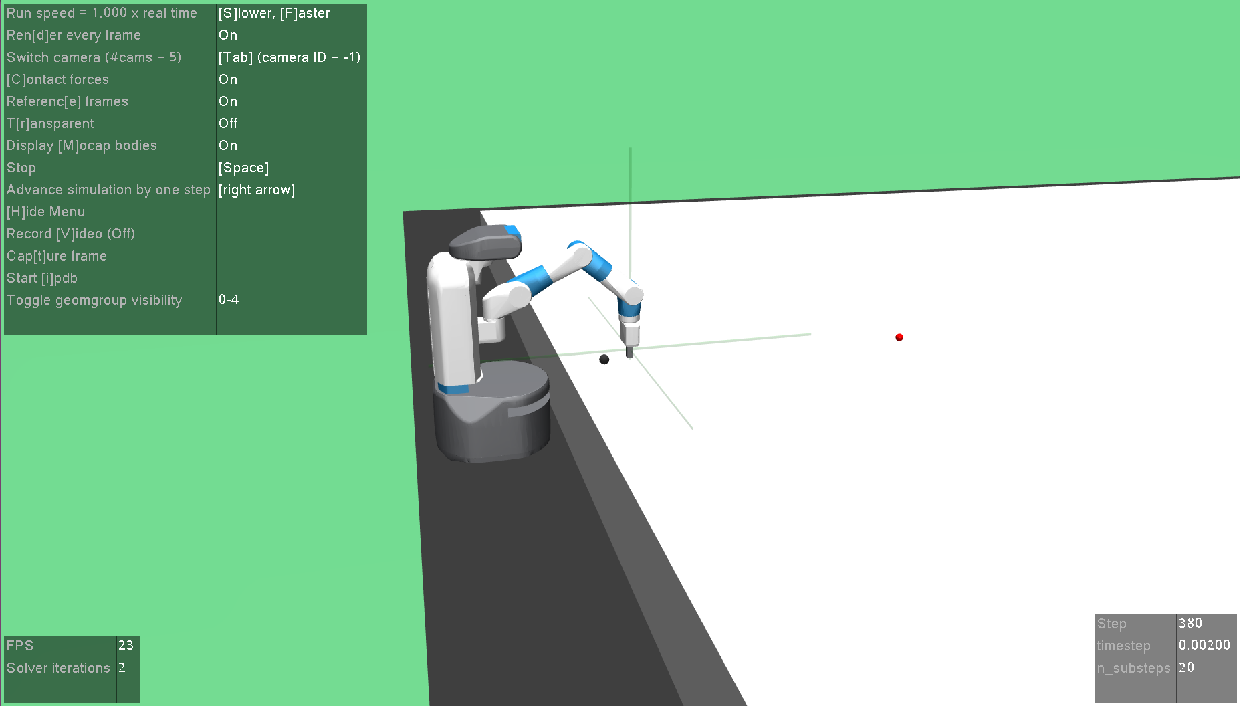
\includegraphics[width=1\textwidth]{figures/FetchSlideball-v3.pdf}
	\caption{FetchSlideball-v3}
	\label{slideball1}
\end{figure}

The environment can be seen in figure \ref{slideball1}. The size of the table was increased drastically. This was done to ensure that the goal would be on the table. The table is just much bigger than necessary to be able to accomodate future environments where the goal will be put in much farther distance. The object is a ball. As usual, there is a fetch robot and a red sphere marking the goal position. 

%put some experiment section for the differennt variables/versions used ?



\subsection{Results}


\begin{figure} [!h]
	
	\centering
	\subfigure[FetchSlide-v1] {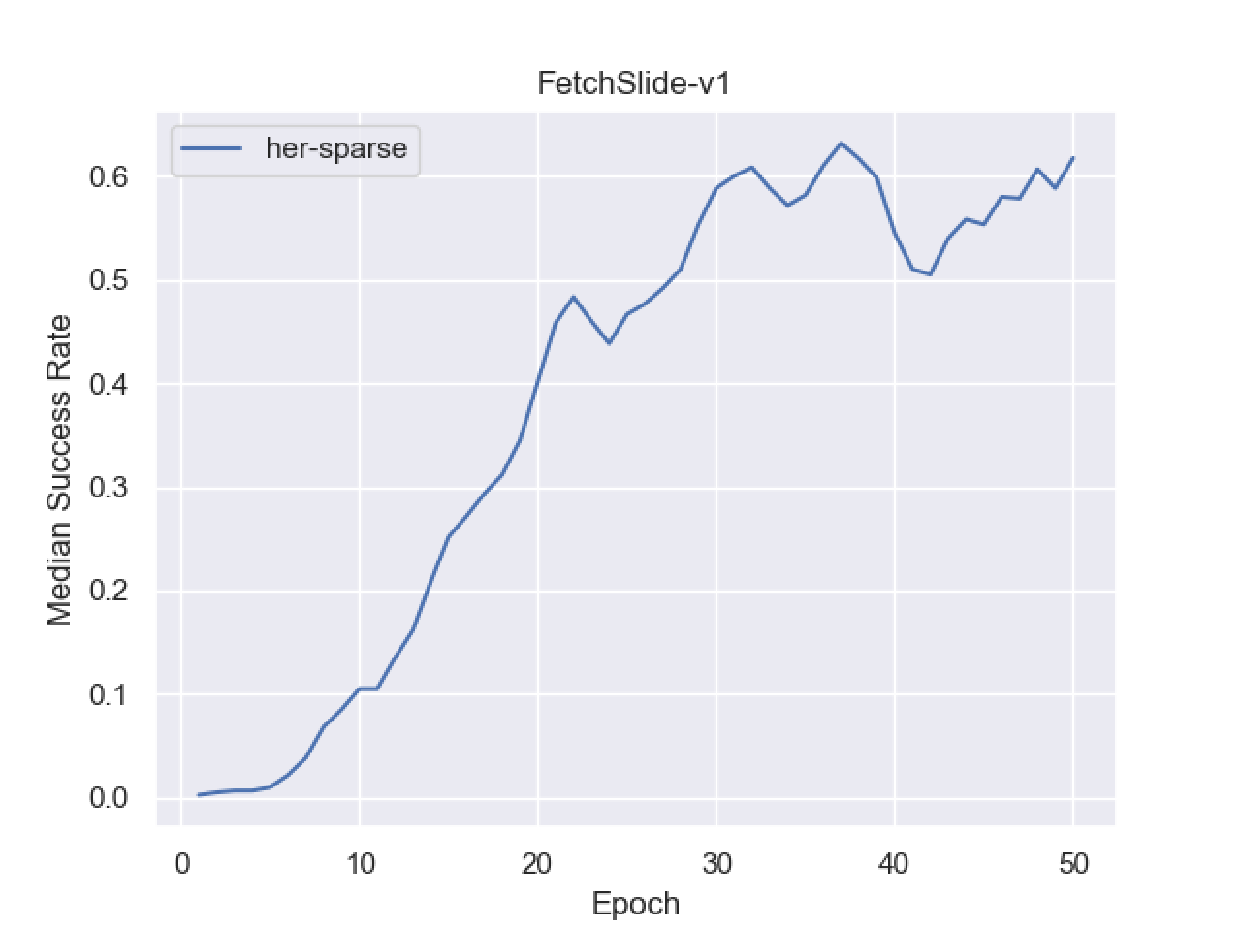
\includegraphics[width=0.49\textwidth]{figures/fig_FetchSlide-v1.pdf}\label{fig:fig_fetchslide-v1}}
	\subfigure[FetchSlideball-v1] {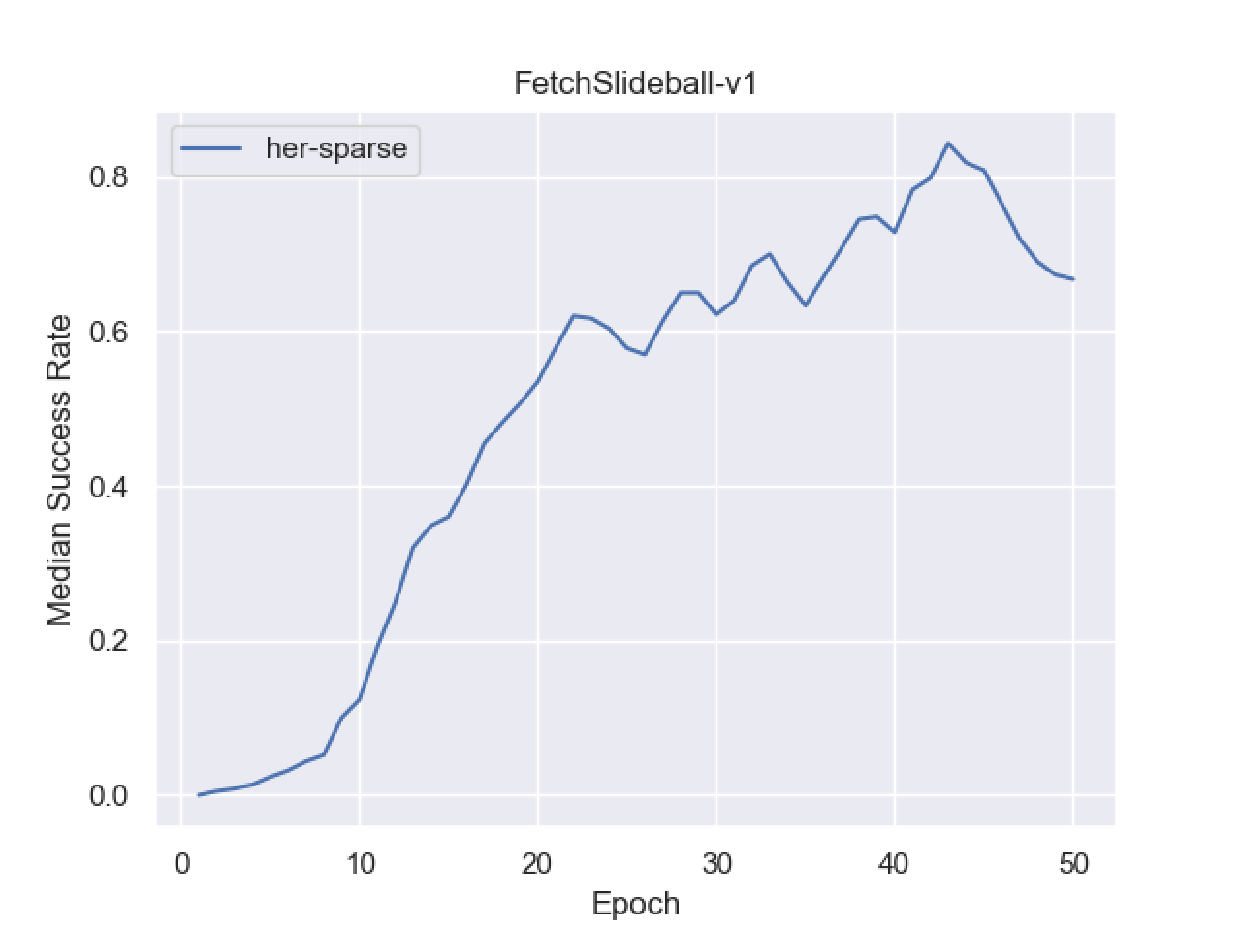
\includegraphics[width=0.49\textwidth]{figures/fig_FetchSlideball-v1.pdf}\label{fig:fig_fetchslideball-v1}}
	\caption{FetchSlide with a cylinder (left) and with a ball (right)}
	\label{slidecomp}
\end{figure}


First the FetchSlide environment was used with the only change being a ball. As can be seen in figure \ref{slidecomp}, FetchSlide with a ball performs much better than vanilla FetchSlide with a cylinder. Both learning curves are quite similar. They both have a success rate curve for the first 20 epochs. After the first 20 epochs, the success rate is still rising, but visibly slower. While FetchSlide with the cylinder only reaches a success rate of 60\%, FetchSlide with a ball reaches about 80\%. The difference might be explained by the ball being more stable. The cylinder that is used in the normal FetchSlide environment can fall over when it is moved at a bad angle, this can not happen to a ball.
%werid explanation, try to find out more
\newline
Afterwards the experiment continues for the FetchSlideball environment with a bigger distance. The new distance from start position of the ball to the goal position is about the doubled distance of the normal FetchSlide environment.
%fill in exact distances.
Training the FetchSlideball environment without changing any of the other parameters proved to be impossible as figure \ref{slideball2} shows. Later it was discovered to be because of a simple reason. The goal is too far away, so it is physically impossible for the robotic arm to roll the ball to the goal.
 
\begin{figure} [h]
	
	\centering
	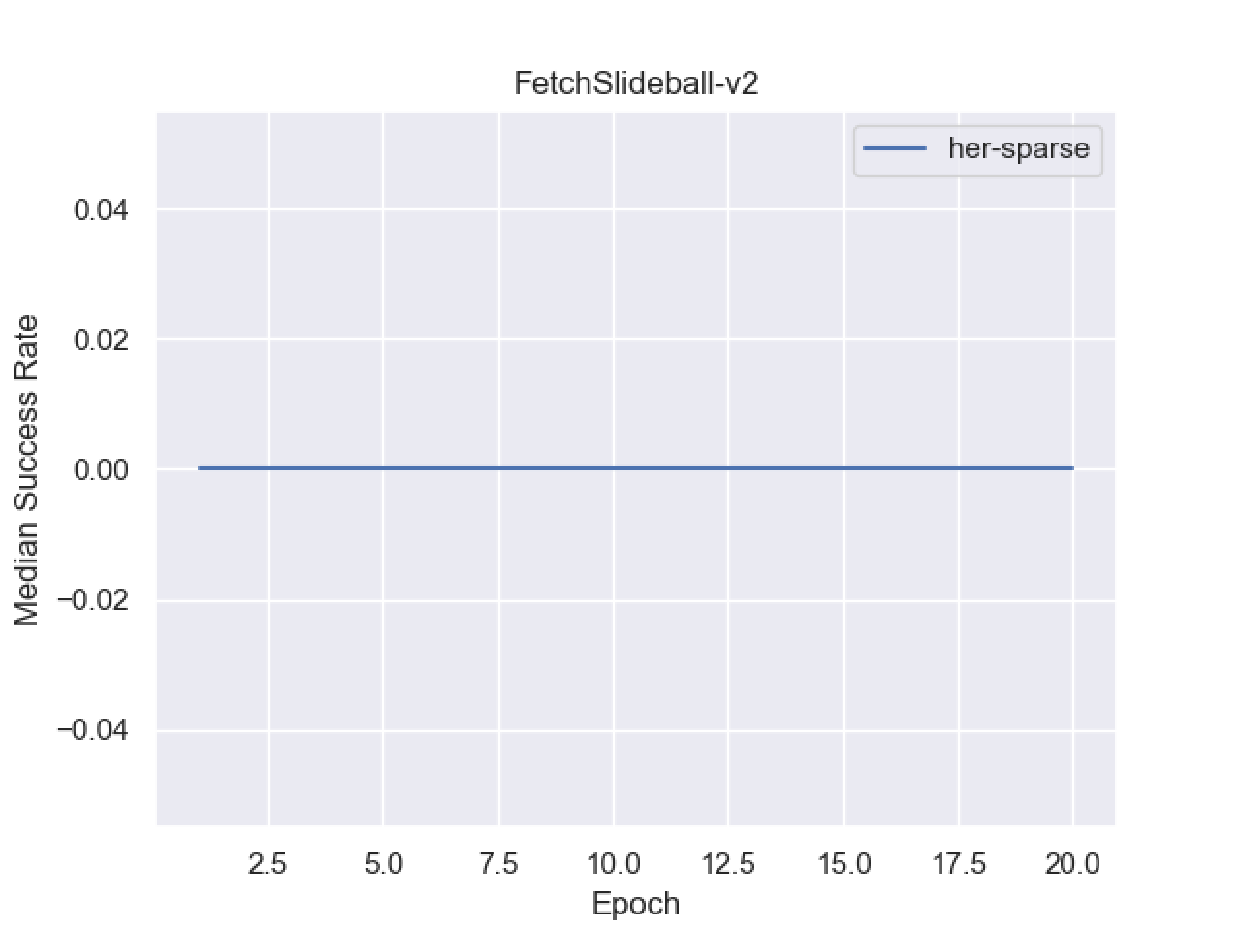
\includegraphics[width=1\textwidth]{figures/fig_FetchSlideball-v2.pdf}
	\caption{FetchSlideball with the same friction and timestep as in FetchSlide}
	\label{slideball2}
\end{figure}

Reducing the friction by 50\% made it barely possible to reach the goal. The goal could be reached, but the goal position is at the limit of the range that the ball could reach. Figure \ref{slideball3} showed how hard it is to learn to reach the goal. For the first 30 epochs, there was no success. Weirdly, at epochs 30 to 34 the goal was reached, but afterwards there was no success again. 
%some randomness ? but 4 episodes in a row ?
%TODO check this, maybe retry the experiment    

\begin{figure} [h]
	
	\centering
	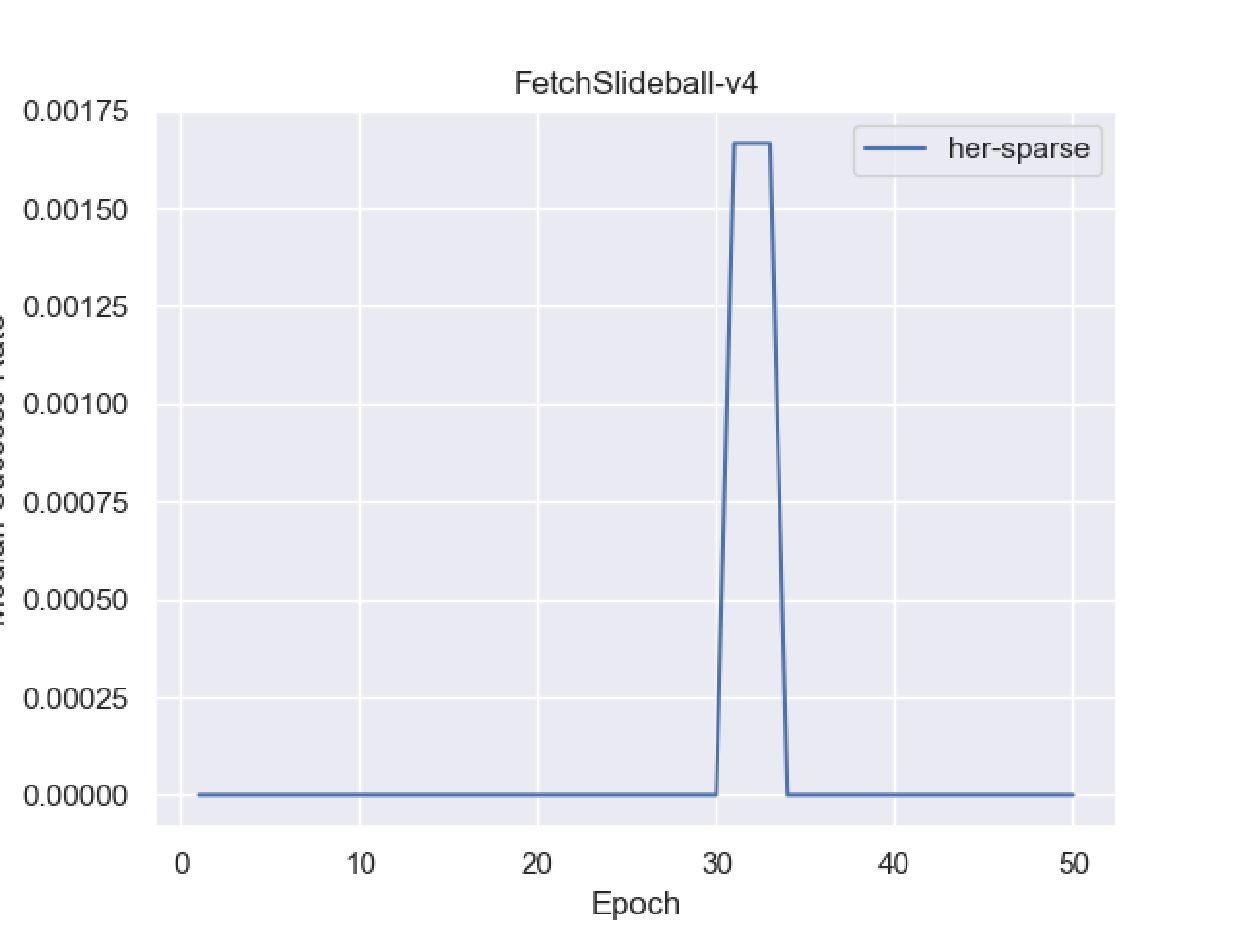
\includegraphics[width=1\textwidth]{figures/fig_FetchSlideball-v4.pdf}
	\caption{FetchSlideball with 50\% friction and more steps per episode}
	\label{slideball3}
\end{figure}

Changing the balls' friction to only 10\% of the original friction showed interesting results. As can be seen in figure \ref{slideball4}, for the first 15 epochs there is no success, but then the success rate slowly rose. At episode 47 the success rate spiked to almost the doubled success rate. The reason behind that shows how tricky the agent can be. Each training episode takes 1000 time steps. The episode is successful when the goal is reached, to be precise, in this environment if the ball is in a close range (0,05 units of length) of the goal position in the last time step.
The agent abuses this fact to solve the task different than intended. The intended solution is to roll the ball with just enough force, so that it stops at the exact goal position and stays there, so that the success condition is fulfilled and the task is successful solved. But the agent uses a different idea. It tries to hit the ball at exactly the right time, so that the ball is just at the goal position at time step 1000, the ball does not need to stop there. If the episode would take more time steps, then the ball would just roll too far, but because the episode ended at 1000 time steps, the success condition is fulfilled and the episode is counted as solved right.
But even in the cases where the episode is not successful, the robotic arm slides the ball in the right direction, it just rolls too far. When using the trained policy of the 10\% friction FetchSlideball environment to solve the task with 50\% friction, it is getting quite close to the goal because it learned to move the ball in the right direction.

%do 25% friction ?

\begin{figure} [h]
	
	\centering
	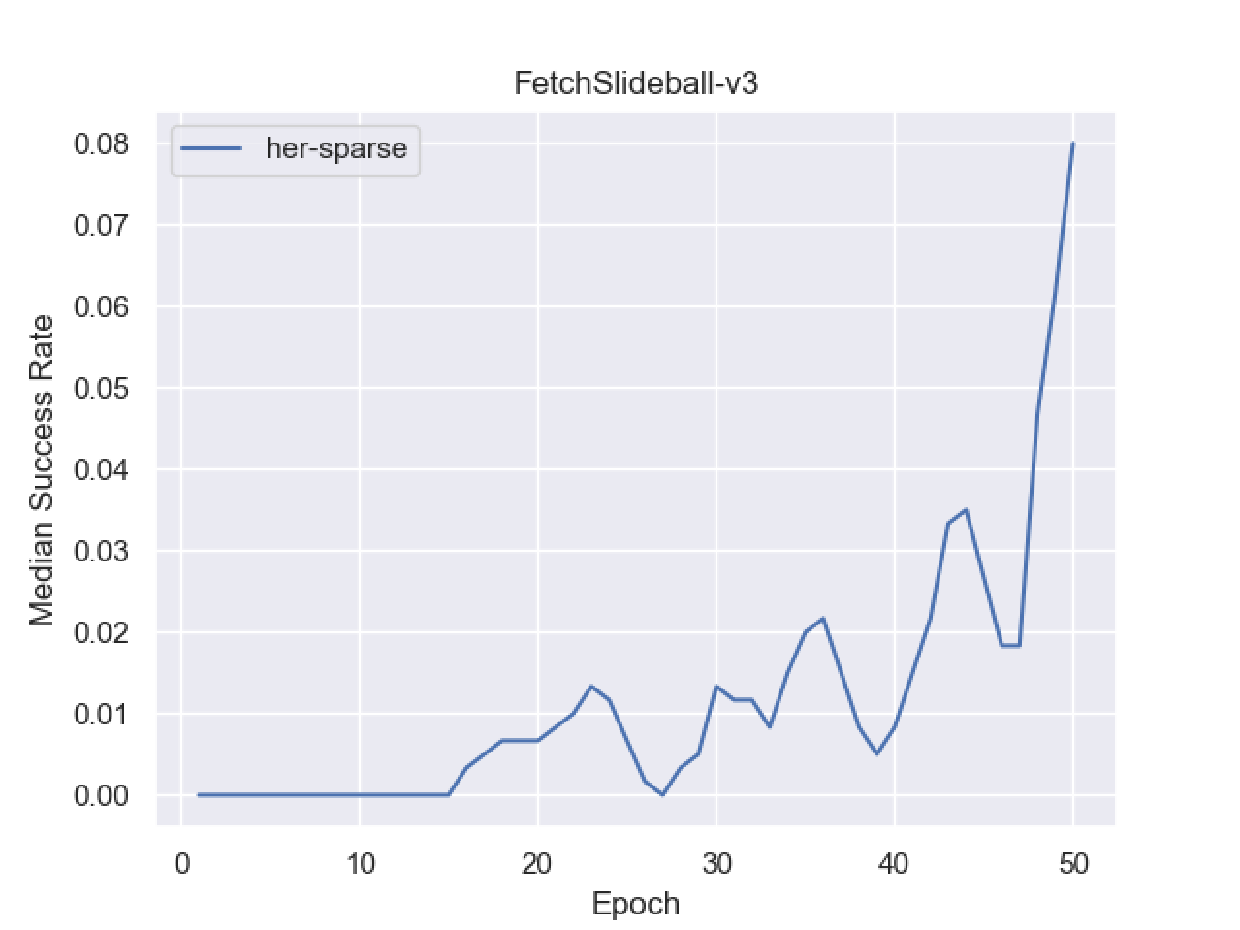
\includegraphics[width=1\textwidth]{figures/fig_FetchSlideball-v3.pdf}
	\caption{FetchSlideball with 10\% friction)}
	\label{slideball4}
\end{figure}

%do 10% friction, more time steps.

\subsection{Discussion}

Through these experiments two findings were learned. Using a ball instead of a cylinder improves the performance of the agent. This is attributed to the ball being a stable object. In this case, the ball showed an improvement of 33\% over the cylinder. It might be interesting to compare the ball to other objects. 
\newline
Also it was figured out that a bigger distance to the goal position increases the difficulty of the task greatly. For the FetchSlideball task with 10\% friction, only 8\% success rate could be reached after 50 episodes in comparison to the 60\% success rate by the FetchSlide task. And even for that 8\% success rate, the agent did not solve the task the intended way. 
\newline
This poses two questions: Is the difficulty solely rising due the fact that the goal distance is increasing or does the difficulty also depend on the proportion between goal distance and range where the robotic arm can roll the ball to? More experiments with different friction values have to be done to answer this question.
\newline
Also, how can the agent be prevented from solving the task in an unintended way ? To really solve the task in the intended way, the implementation of the task needs to be changed. The FetchSlideball task needs to change to have the ball lie on the goal position for some time, to count the task as successfully solved. This would prevent a ball that only touches the goal at the end to be counted.
\newline
The results have shown that vanilla HER can not solve these tasks where we increased the goal distance far outside the robotic arms' reach. To solve these tasks, further experiments with improved HER algorithms like Hindsight Goal Generation need to be done. As stated by Ren et al. \cite{hgg}, many hindsight experiences are not helpful to replay and therefore the hindsight goals need to be selected better to improve the performance. Especially in the case of the task FetchSlideball with 50 \% friction, the goal was located at the edge of the range where the robotic arm can roll the ball to. An approach where the agent is guided to roll the ball more often in the direction of the goal would improve the performance. Further research with improved HER approaches will be done in the future.

\section{FetchToss}

FetchToss is rather different than the other environments. For future plans, FetchToss is planned to become an environment that resembles basketball. The agent should learn how to throw a ball into a basket. This environment has similarities to FetchPickAndPlace and FetchSlide, because the gripper has to be used to grab a ball and the goal is also outside of the robotic arms' range. To solve the task, we first try to change the object to a ball and see how picking a ball compares to picking a cube.
Then a box is used to try to make the agent learn, how to toss the ball into the box.

\subsection{Task Description}

The task for FetchToss is to fetch a ball that is placed on the table and toss it into a box that is not reachable by the robotic arm without tossing. The goal has to be outside of reach to avoid having the robot just picking the ball up and putting it inside. The goal position and size is different than for the other tasks. For one, the goal this time is static, it will always be the same box at the same position. Also, the goal is much bigger this time. The task is fulfilled, when the ball is inside the box, it does not matter where in the box. The red sphere is just a visual mark, the actual goal is the whole box. The agent has to learn following steps: Pick up the ball like in FetchPickAndPlace, then move the object with enough force towards the goal and open the gripper to toss the ball and also hit the goal.


\subsection{Environment}

\begin{figure} [ht]
	
	\centering
	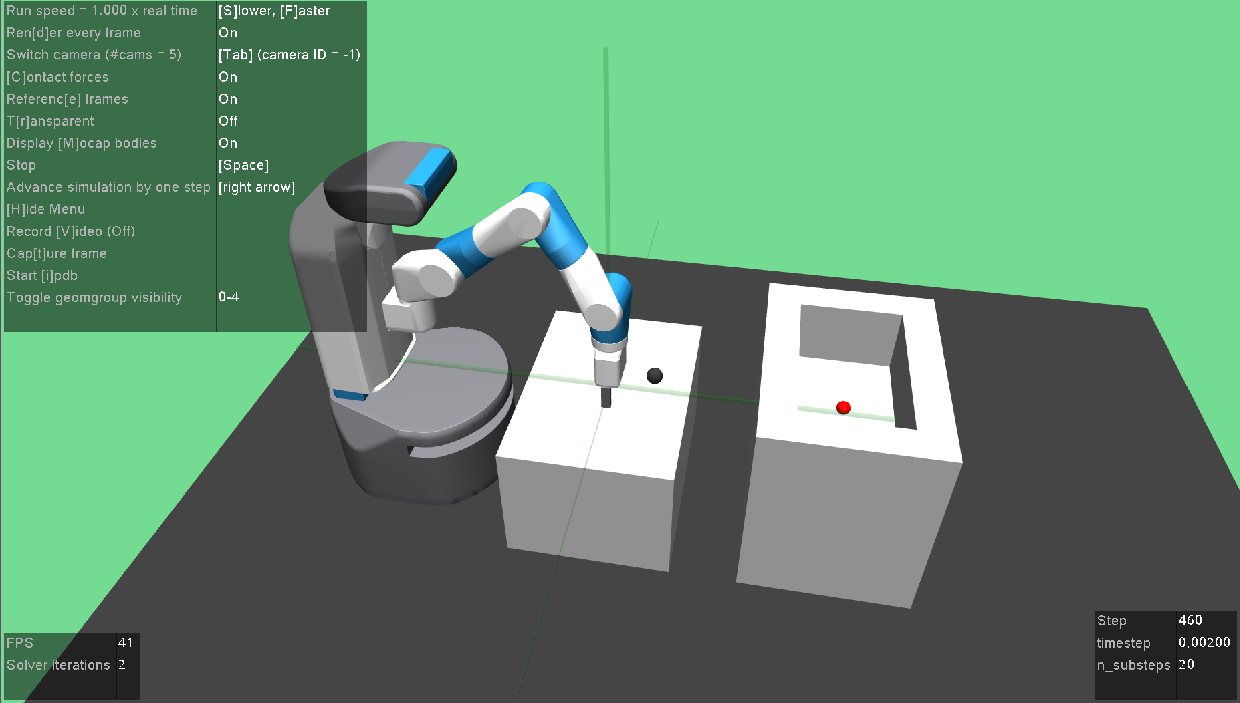
\includegraphics[width=1\textwidth]{figures/FetchToss-v1.pdf}
	\caption{FetchToss}
	\label{toss1}
\end{figure}

For this environment the environment of FetchPickAndPlace was used as a base. The object was also changed into a ball and a box was created to simulate as basket. As usual, there is also a fetch robot and a red sphere marking the goal. As mentioned, the actual goal contains the whole box, not only the position of the red sphere. Also, the goal is static.

\subsection{Results}

\begin{figure} [!ht]
	
	\centering
	\subfigure[FetchPickAndPlace-v1] {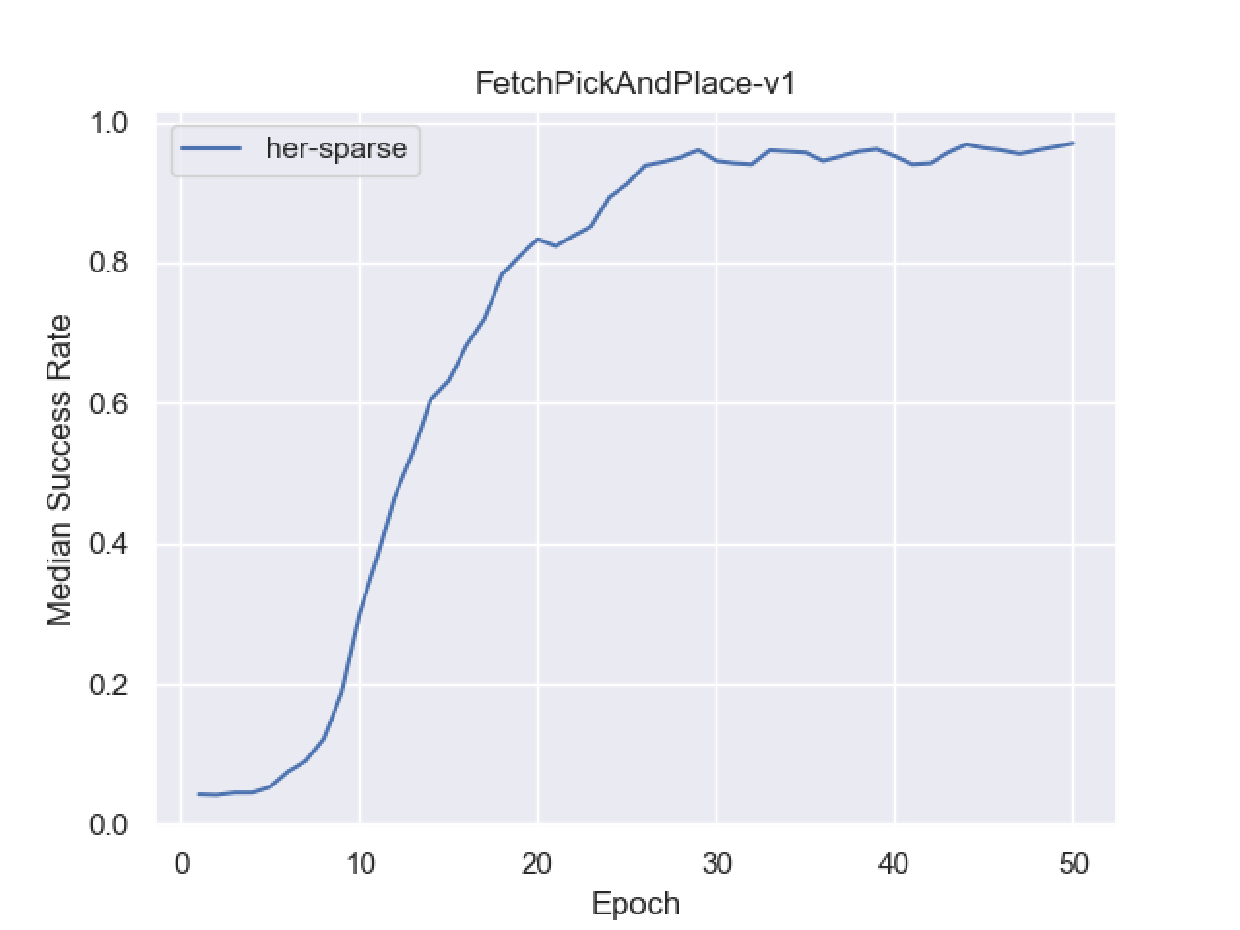
\includegraphics[width=0.49\textwidth]{figures/fig_FetchPickAndPlace-v1.pdf}\label{fig:fig_fetchpickandplace-v1}}
	\subfigure[FetchPickAndPlaceball-v1] {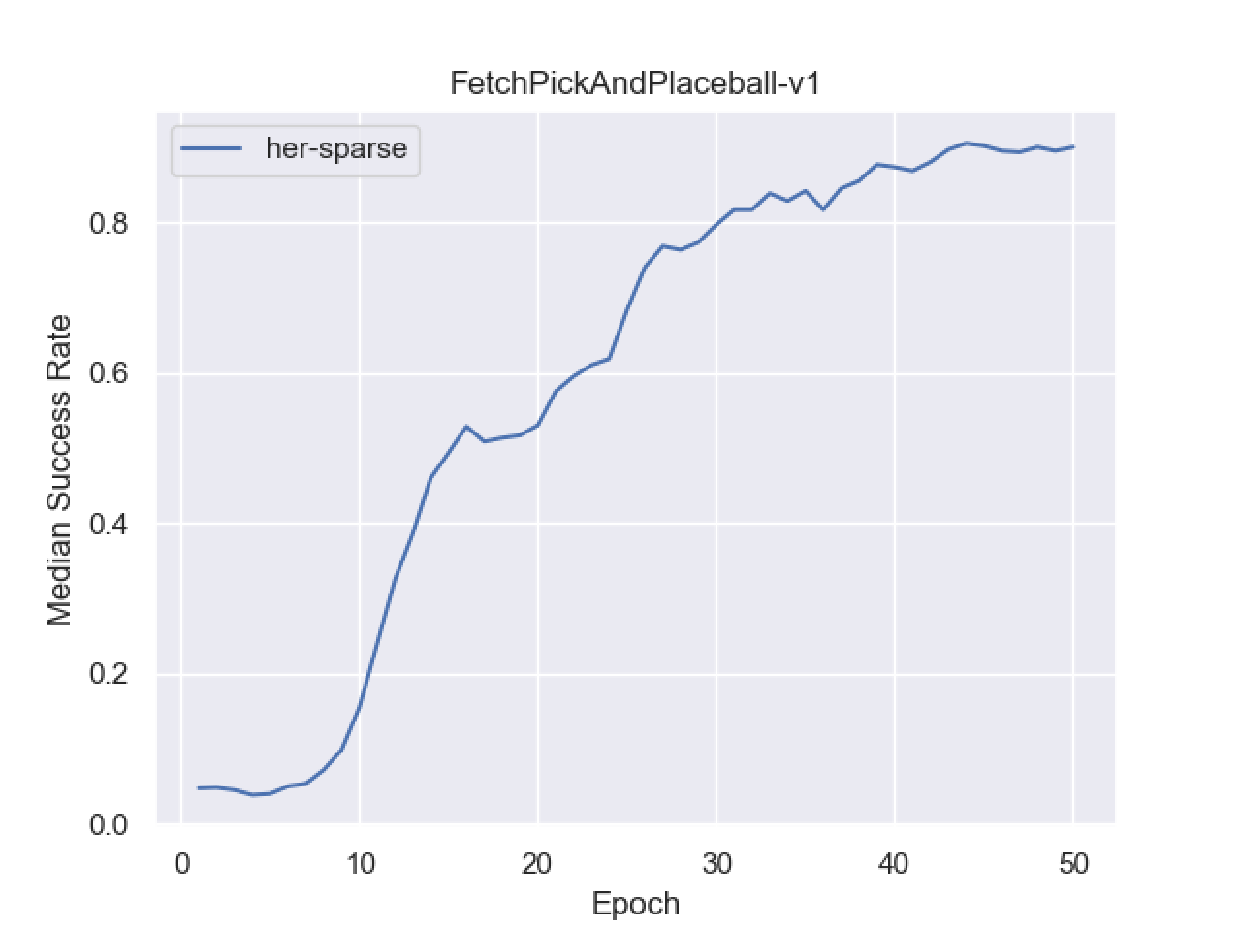
\includegraphics[width=0.49\textwidth]{figures/fig_FetchPickAndPlaceball-v1.pdf}\label{fig:fig_fetchpickandplaceball-v1}}
	\caption{FetchPickAndPlace with a cube(left) and a ball (right)}
	\label{pickballcube}
	
\end{figure}

As figure \ref{pickballcube} shows, picking up a ball instead of a cube seems to perform worse. Both show similar success rate curves. FetchPickAndPlaceball seems to differ at about epoch 15. While FetchPickAndPlace still has a steep success rate curve at epoch 15, FetchPichAndPlaceball already slows down with being more successful. Overall FetchPickAndPlace with the ball shows slightly lower success rates. While it reaches about 90\% success rate at 50 epochs, the vanilla FetchPickAndPlace with the cube reaches about 95\% success rate.

\begin{figure} [!ht]
	
	\centering
	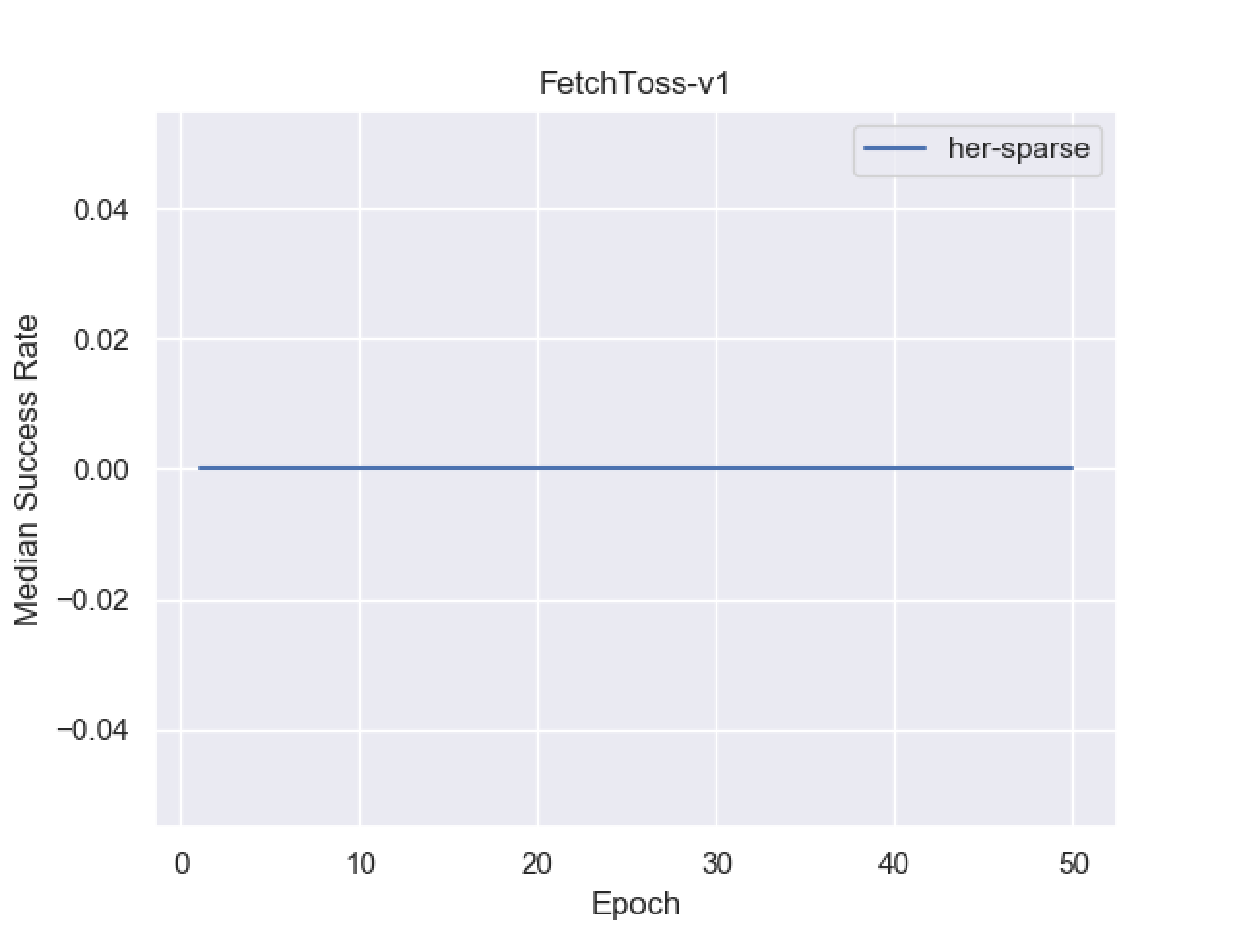
\includegraphics[width=1\textwidth]{figures/fig_FetchToss-v1.pdf}
	\caption{FetchToss}
	\label{toss2}
\end{figure}

Figure \ref{toss2} summarizes the results for the other experiments that were run. The robotic arm does not learn how to toss the ball at all. The box was changed to a box where the front is open to make it easier to toss in the back was made higher to prevent the agent from throwing the ball over the box. This also showed the same results. Another try was lengthening the time steps per episode from 1000 time steps to 2000 time steps, because it could just be impossible to solve the task as tossing takes some time. The ball was also made 100 times lighter (from 2 to 0.02 units of weight) which did not change the result. A path was planned manually to show if the reason for failing might be because the task itself is impossible. For the environment with the lighter ball a path to solve the task is possible which can be seen in Figure \ref{toss3}. This means that vanilla HER can not solve this task. Also tossing a cube instead of the ball does not work. This also proved to be unsuccessful. 

\begin{figure} [!h]
	
	\centering
	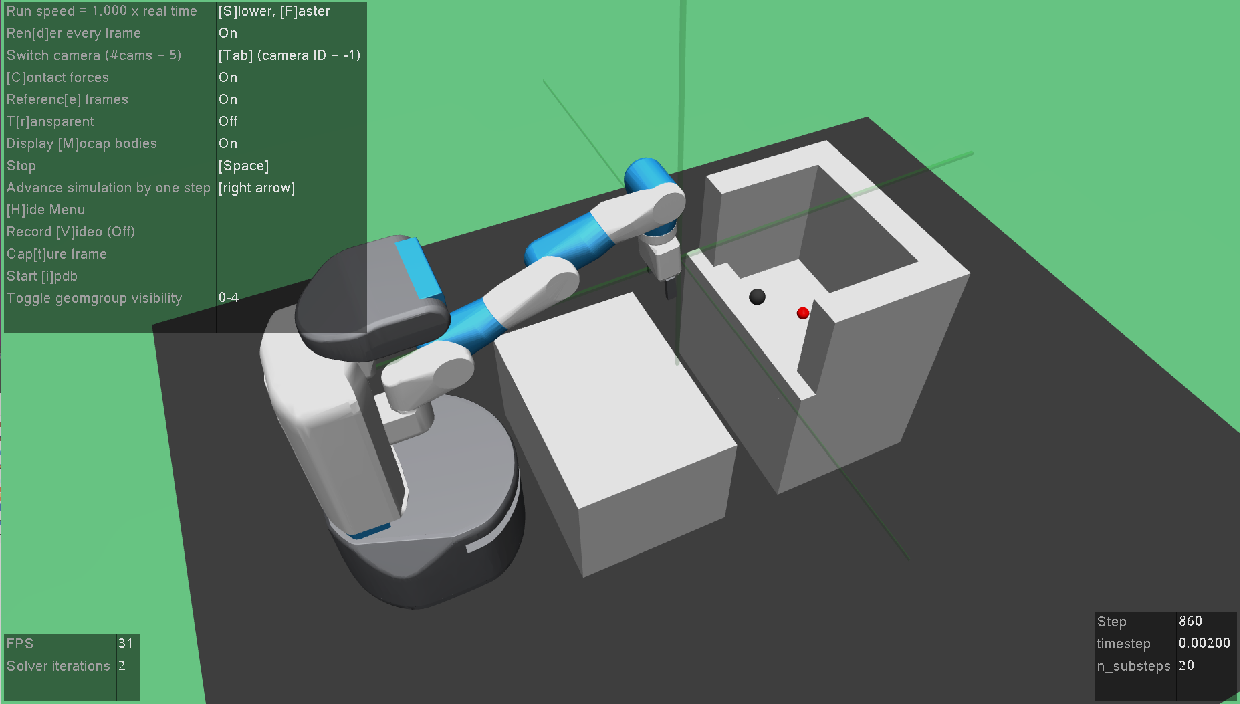
\includegraphics[width=1\textwidth]{figures/FetchToss-v0.pdf}
	\caption{FetchToss, with lighter ball and more time steps}
	\label{toss3}
\end{figure}

\subsection{Discussion}

Picking up a cube seemed to be easier than the ball. A reason might be because of their size form. A ball with radius of 0,02 units of length, and therefore a diameter of 0,04 units of length is simply smaller than a cube with each side being 0.04 units of length long. Even though both objects have 0,04 units of length at their longest part, the ball is just smaller. Also, because of the balls form, is has to be grabbed at the middle while the cube can be grabbed at any side, it will always be 0,04 units of length long. The cube is just easier to grab and harder to drop than a ball. Experiments could be done to figure out how big the ball has to show as much success as for the cube.
\newline 
Learning to toss the ball is pretty difficult as the results show. It was proven that the task is physically possible by finding a path for the lighter ball. So it seems that the task of tossing a ball is too hard to learn with standard HER.
\newline
As explained by Ren et al. \cite{hgg}, HER has the flaw that it learns how to solve goals that are equal to states that the agent already reached once, even though these goals might not be useful to learn how to solve the actual goal. In the FetchToss task learning how to toss the ball in the box seems to take too many difficult steps to learn. So vanilla HER fails. Improved HER algorithms might be useful to solve the task. Especially the energy-based hindsight experience prioritization approach by Zhao and Tresp \cite{energyher} might be useful for this task because tossing requires a lot of energy and therefore prioritizing replaying experiences with high energy would be especially fitting.
Further research in this direction will be done in the future.



